\documentclass[11pt]{article}
\usepackage[margin=1in]{geometry}
\usepackage{amsmath,amssymb,booktabs,graphicx,setspace,caption,hyperref}
\usepackage[T1]{fontenc}
\usepackage{mathpazo}
\setlength{\parindent}{0pt}
\setlength{\parskip}{0.6em}
\captionsetup{font=small,skip=6pt}
\title{Panel MS-AR(1) from 1995: common RW trend and RE intercepts\\[0.4em]\large Seasonally adjusted real GDP per worker}
\author{}
\date{}
\begin{document}
\maketitle
\section{Model}
Sample starts in 1995Q1. Two-step. Step 1 is a common trend from average growth of countries observed in consecutive quarters:
\begin{align}
\Delta\tau_t &= \frac{1}{n_t^{\mathrm{cont}}}\sum_{i\in C_t\cap C_{t-1}} (y_{it}-y_{i,t-1}), \\
\tau_t &= \tau_{t_0}+\sum_{s=t_0+1}^{t}\Delta\tau_s.
\end{align}
The level of $\tau$ is pinned to the balanced-core mean at $t_0$. Mean $\Delta\tau$ is 0.0041 per quarter (3 countries present in every quarter). Step 2 is estimated on $y_{it}^\ast=y_{it}-\hat\tau_t$:
\begin{align}
y_{it}^\ast &= a_i + z_{it}, \\
a_i &\sim \mathcal{N}(\alpha,\omega^2), \\
z_{i,t+1} &= \bigl(1-\rho(s_{it})\bigr)\mu(s_{it}) + \rho(s_{it})\, z_{it} + \sigma(s_{it})\,\varepsilon_{it}.
\end{align}
No catch-up term. No extra $gt$. Three regimes; median $\mu$ pinned at 0; $\sigma$ and $\rho$ switch; $|\rho|<0.99$. Random intercepts: 11-point Gauss--Hermite. Plotted cycles use posterior-mean $a_i$. $\tau_t$ is discarded for the structural MS-AR. Standard errors ignore step-1 uncertainty.
\begin{figure}[h]
\centering
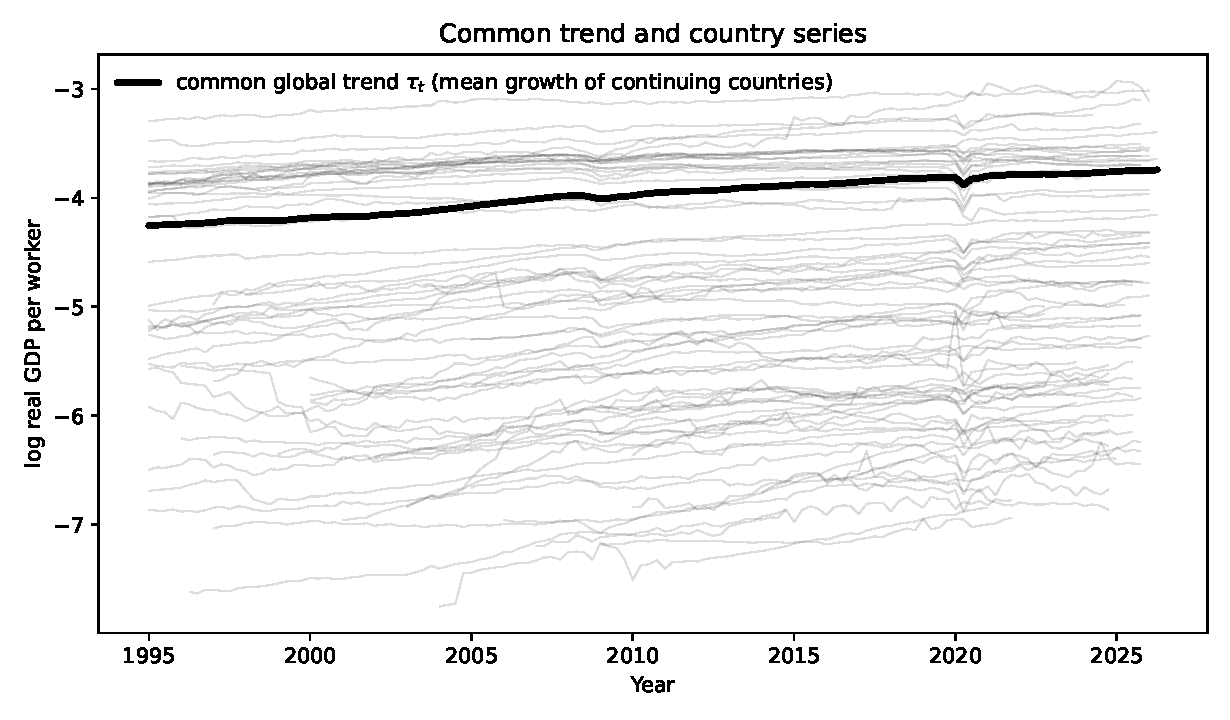
\includegraphics[width=0.88\textwidth]{figs/tau_rw_1995.pdf}
\caption{Faint lines: country log real GDP per worker. Thick line: common $\tau_t$ from average growth of continuing countries.}
\end{figure}
\clearpage
\section{RE intercepts around the common RW trend (no catch-up)}
2026-09-17 SA panel, $y_{it}=a_i+\tau_t+z_{it}$, from 1995. 74 countries, 7648 observations, 1995-Q1--2026-Q2. $|\rho|<0.99$. Fitted countries: 74. Observations: 7648. Log-likelihood: 20676.70. Ergodic mean of the cycle $E[z]=0.0694$ (0.0236).
Random intercepts $a_i\sim N(\alpha,\omega^2)$ with $\alpha=-0.6457$ (0.0114), $\omega=0.6738$ (0.0072). Posterior-mean $a_i$: mean -1.155, min -3.298, max 0.618.
\begin{table}[h]
\centering
\caption{Regime AR(1), transition matrix, and ergodic $\pi$. Columns are regimes.}
\begin{tabular}{lccc}
\toprule
 & (0) & (1) & (2) \\
\midrule
$\mu$ & -0.5317 & 0.0000 & 0.2928 \\
 & (0.1067) & --- & (0.0260) \\ \addlinespace
$\sigma$ & 0.0719 & 0.0074 & 0.0190 \\
 & (0.0029) & (0.0001) & (0.0005) \\ \addlinespace
$\rho$ & 0.9897 & 0.9900 & 0.9900 \\
 & (0.0039) & (0.0000) & (0.0000) \\ \addlinespace
$\Pi_{0\cdot}$ & 0.6740 & 0.0000 & 0.3260 \\
 & (0.0375) & (0.0001) & (0.0375) \\ \addlinespace
$\Pi_{1\cdot}$ & 0.0095 & 0.9438 & 0.0467 \\
 & (0.0032) & (0.0056) & (0.0062) \\ \addlinespace
$\Pi_{2\cdot}$ & 0.0622 & 0.0676 & 0.8701 \\
 & (0.0082) & (0.0077) & (0.0112) \\ \addlinespace
$\pi$ & 0.0930 & 0.4954 & 0.4116 \\
 & (0.0103) & (0.0258) & (0.0221) \\ \addlinespace
\bottomrule
\end{tabular}
\end{table}
\begin{figure}[h]
\centering
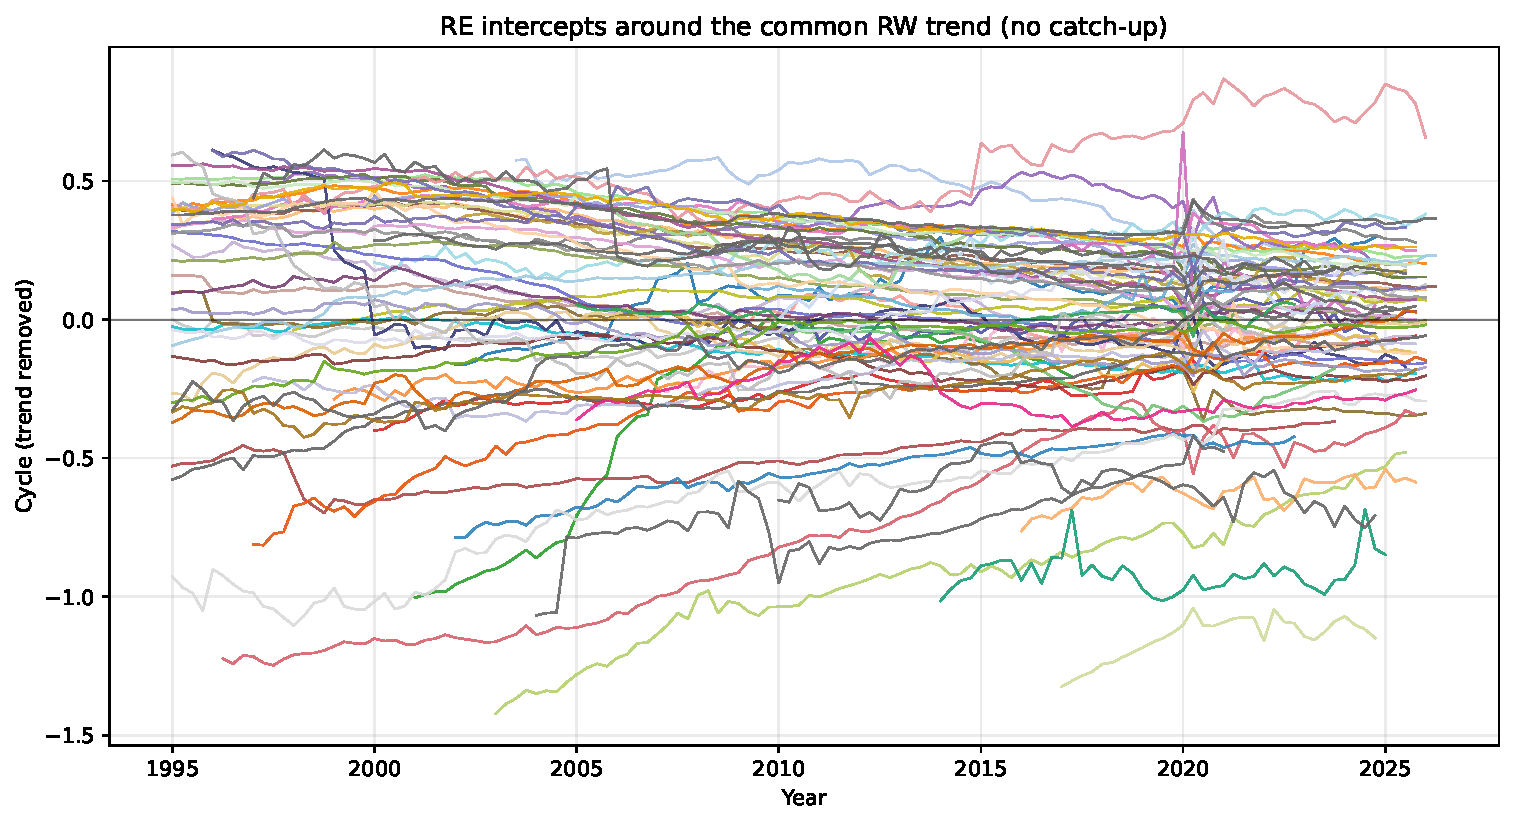
\includegraphics[width=0.75\textwidth]{figs/cycle_rw1995_re.pdf}
\caption{Country cycles after removing $\tau_t$ and posterior-mean $a_i$.}
\end{figure}
\end{document}
